\documentclass[12pt]{article}
\usepackage[left=2cm,top=2cm,right=2cm,bottom=2cm]{geometry}
\usepackage[parfill]{parskip}
\usepackage{amsmath}
\usepackage{graphicx}
\usepackage{listings}
\lstloadlanguages{python}
\usepackage{amssymb}
\usepackage{braket}
\usepackage{pdfpages}
\usepackage{hyperref}
\usepackage{cleveref}
\usepackage{float}
\usepackage{physics}
%\usepackage{minted}
%\usemintedstyle{pastie}


\begin{document}
    \begin{titlepage}
        \begin{center}
            \vspace*{5cm}
            
            \Huge
            \textbf{Milestone 1}
            
            \vspace*{0.5cm}
            \LARGE
            AST5220
        
            \vspace*{0.5cm}
        
            \textbf{Julie Thingwall}
        \end{center}
    \end{titlepage}

\section{Introduction}
    In this projet the aim is to numerically reproduce the power spectrum obtained by the CMB data. This will be done in several steps, where each step simulates the different physical processes that make up the power spectrum.
    
    The first step is to model the background cosmology, how the universe and its contents evolve in time without any perturbations. This will be done by utilizing the \textit{very impressive and user friendly} C++ code base provided by our lecturer Hans Winther.



\section{Theory}
\subsection{The Friedman equation and density components}
General relativity tells us, in short terms, that if put stuff with matter or energy in space, then space will change, bend and behave interesting, depending on the nature of the stuff we put in. Using GR, it is possible to obtain expressions that describes how space behaves, given its stuff. 

One such expression is the first Friedman equation. It tells us how the universe as a whole evolves in time, given some density components. It reads as 

\begin{equation}\label{eq:Friedmann Equation}
    H = H_0\sqrt{\left(\Omega_{b,0} + \Omega_{CDM,0}\right)a^{-3} + \left(\Omega_{\nu,0} + \Omega_{r,0}\right) a^{-4} + \Omega_{k,0} a^{-2} + \Omega_{\lambda,0}},
\end{equation}

where $H=\frac{\dot{a}}{a}$ is the Hubble parameter, $H_0$ is the Hubble parameter today, and the $\Omega_{x}$s are the different relative density components of the universe, namely baryons, cold dark matter, neutrinos, radiation, curvature and dark energy respectively. The 0-subscripts means the value of the relative densities today.  $a(t)$ is the scale factor, which measures the size of the universe relative to today. Further on, we will assume a spatially flat universe with no neutrinos, such that $\Omega_k = \Omega_{nu} = 0$.

In general, the relative densities are defined as 

\begin{equation}\label{eq:omega def}
    \Omega_x = \frac{\rho_x}{\rho_c}
\end{equation}

where $\rho_x$ is the density of that given component, and $\rho_c = \frac{3H}{8\pi G}$ is the critical density. 

How the $\rho_x$ in \cref{eq:omega def} evolves in time is governed by the continuity equation 

\begin{equation}
    \dot{\rho} + 3H\rho(1 + \omega) = 0
\end{equation}

where $\omega = \frac{P}{\rho}$ is the equation of state. Solving this equation with respect to $a$ yields 
\begin{equation}\label{eq:density time evolution}
\rho = \rho_0 a^{-3(1+\omega)}.
\end{equation}

For matter (baryons and dark matter), $\omega = 0$. For radioation, it is $\omega = 1/3$ and for dark energy, it is $\omega = 0$. 

Inserting \cref{eq:density time evolution} into \cref{eq:omega def} for each component, and doing some mathemagics, we end up with the four equations defined in \cref{eq:Density parameters}. These equations describes how each component evolves in time. 

\begin{align}\label{eq:Density parameters}
    \begin{split}
    \Omega_b(a) &= \frac{\Omega_{k,0}}{a^3 H^2/H_0^2}  \\
    \Omega_{CDM}(a) &= \frac{\Omega_{CDM,0}}{a^3 H^2/H_0^2}  \\
    \Omega_r(a) &= \frac{\Omega_{k,0}}{a^4 H^2/H_0^2}  \\
    \Omega_{\lambda}(a) &= \frac{\Omega_{k,0}}{H^2/H_0^2} 
    \end{split}
\end{align}

\subsection{Conformal Time}

\begin{equation}\label{eq:Conformal time integral}
    \eta(a) = \int_0^a \frac{c}{a\mathcal{H}}\textrm{d}a
\end{equation}





\section{Implementation}

\section{Results}

\begin{figure}[h]
    \centering
    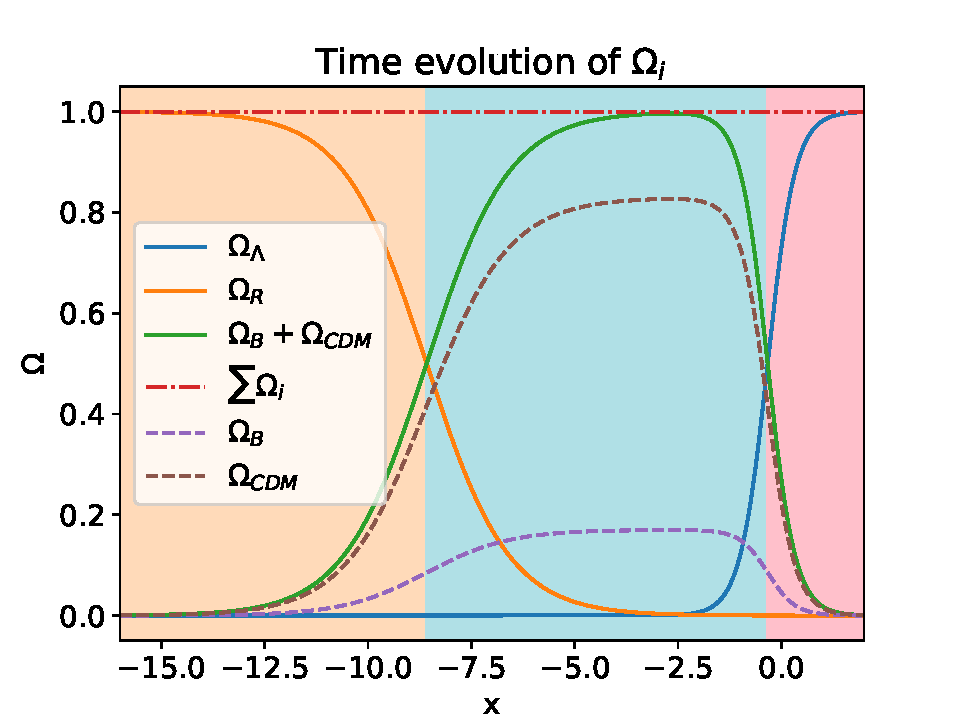
\includegraphics[width=0.9\textwidth]{omega_plot.pdf}
    \caption{Plot showing how the different density parameters evolve as a function of x. The radiation dominated era, matter dominatied era and dark matter dominated era are indicated by the yellow, blue and red background colors respectively.}
    \label{fig:omega}
\end{figure}

\begin{figure}[h]
    \centering
    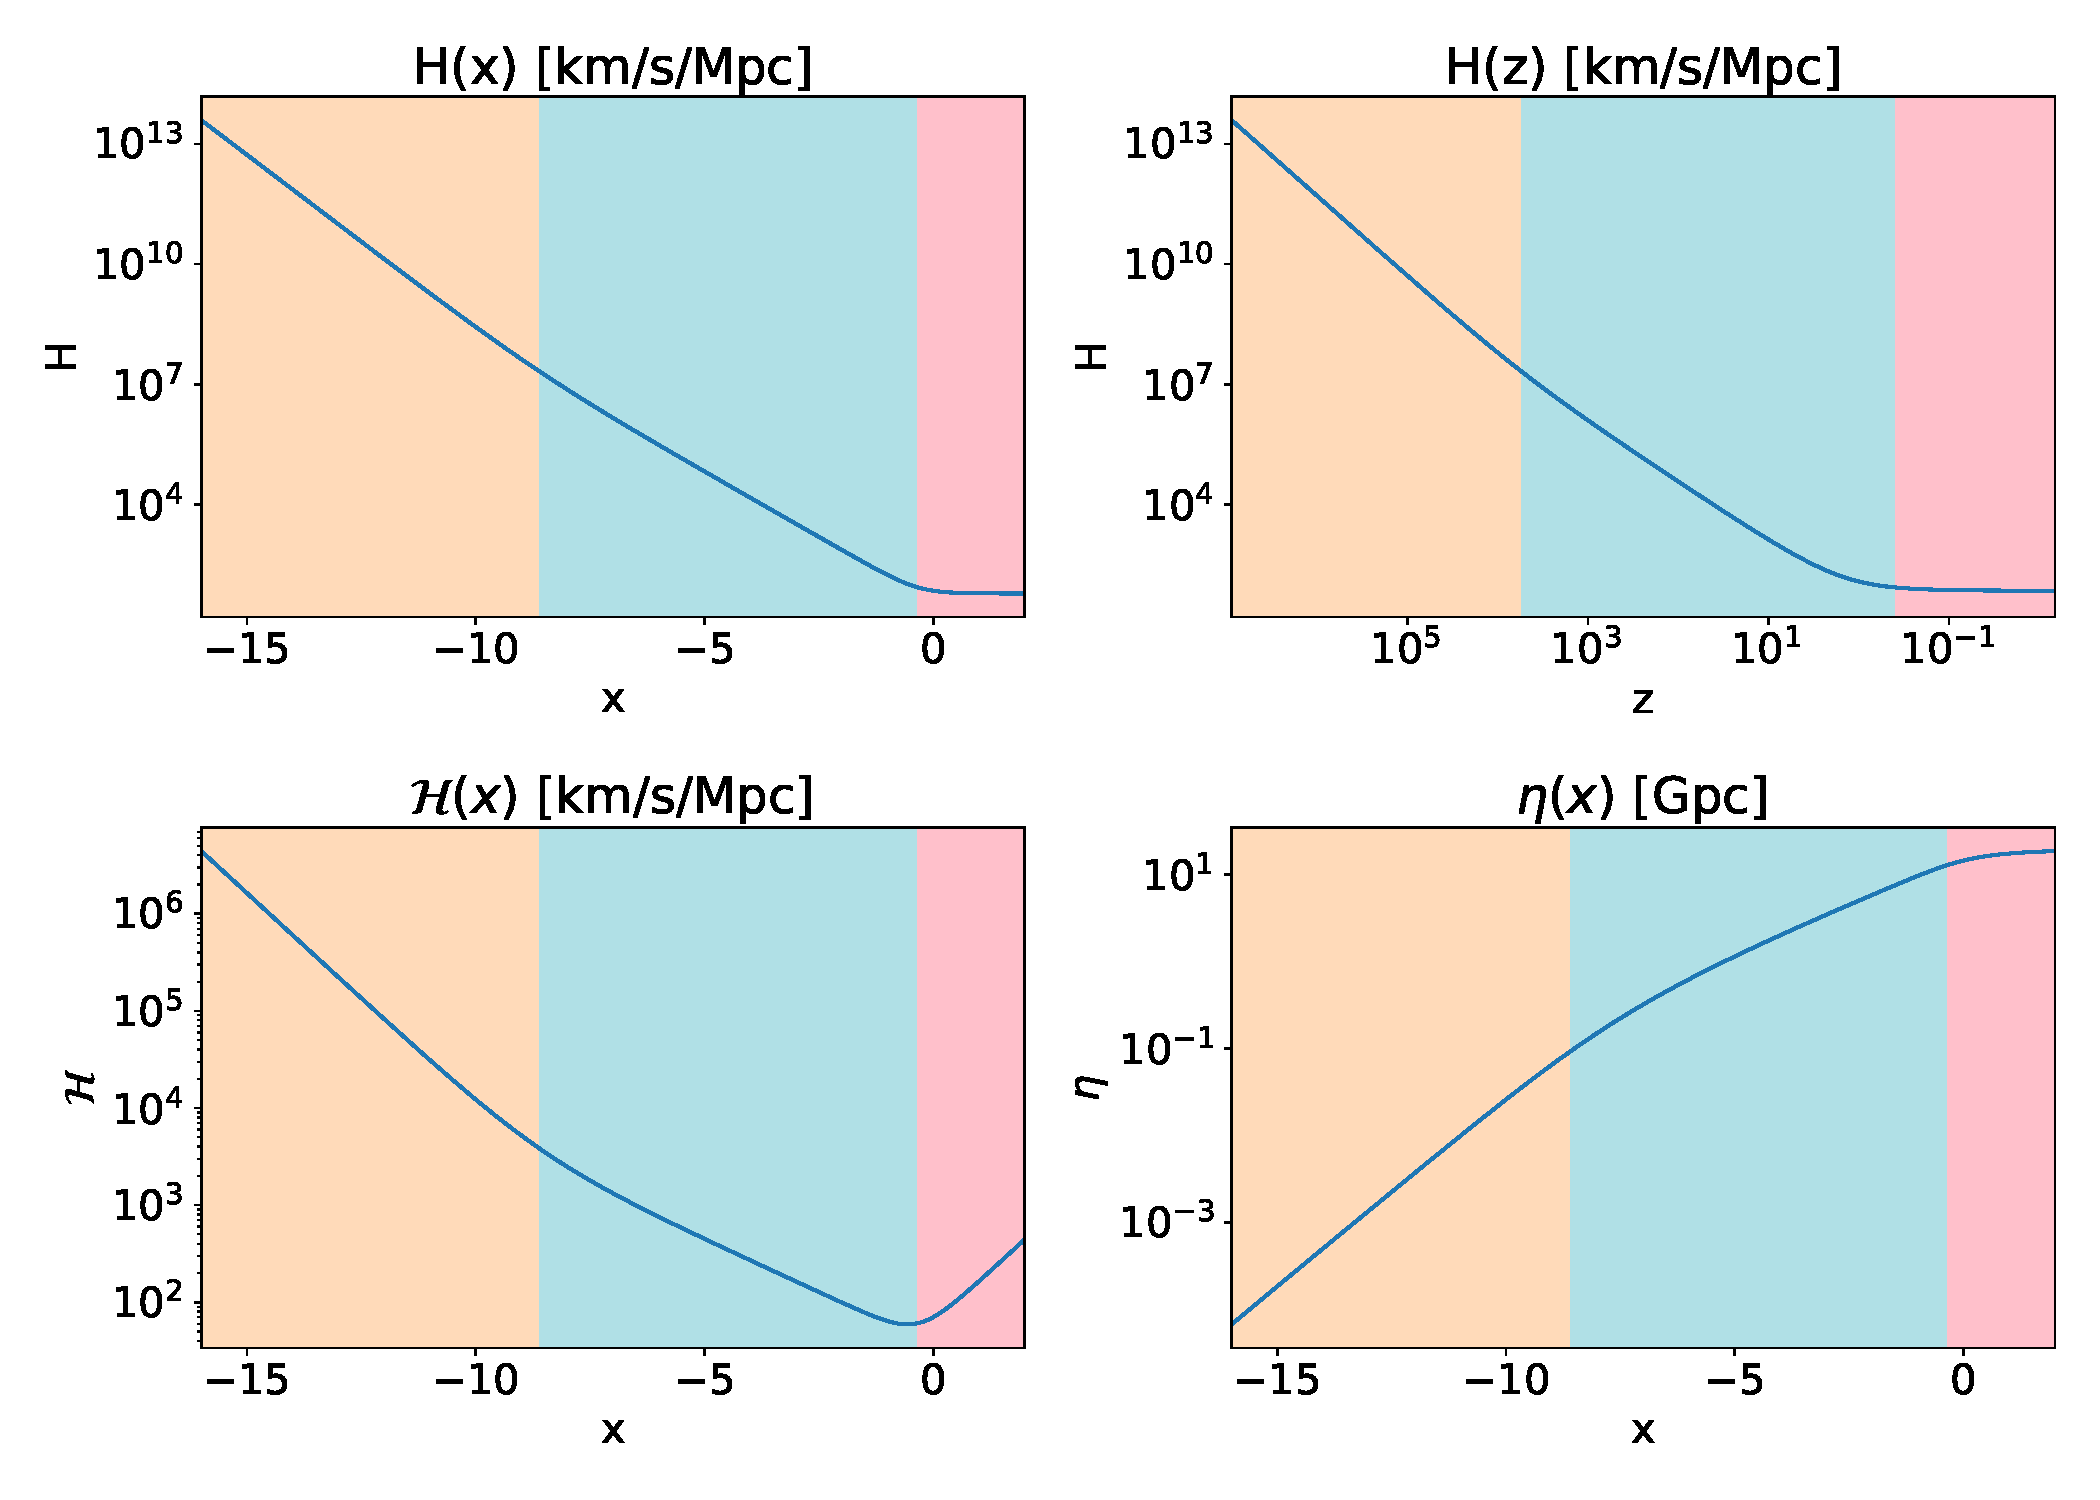
\includegraphics[width=0.9\textwidth]{H_eta_plots.pdf}
    \caption{Plots showing how the Hubble parameter and the conformal time $\eta$ evolves in time. The two upper figures show how the Hubble parameter evolves with respect to $x$ and the cosmological redhist $z$. The lower left picture shows how $\mathcal{H}$ evolves as a function of x. The lower right shows the evolution of $\eta(x)$. As in \cref{fig:omega}, the background colors indicate the different eras of the universe.}
    \label{fig:H_eta}
\end{figure}

\section{Conclution?}



\end{document}